\documentclass[border=5pt,tikz]{standalone}
\usepackage{amsmath}
\usetikzlibrary{calc}
\usetikzlibrary{math}
\usetikzlibrary {shapes.geometric} % for star
\usetikzlibrary{bending} % for arrow head angle
\usetikzlibrary{angles,quotes} % for pic (angle labels)
\usetikzlibrary{arrows.meta} % for arrow size
\usetikzlibrary{decorations.pathmorphing,patterns}

\usetikzlibrary {arrows}
\usetikzlibrary{shapes.geometric}
\begin{document}
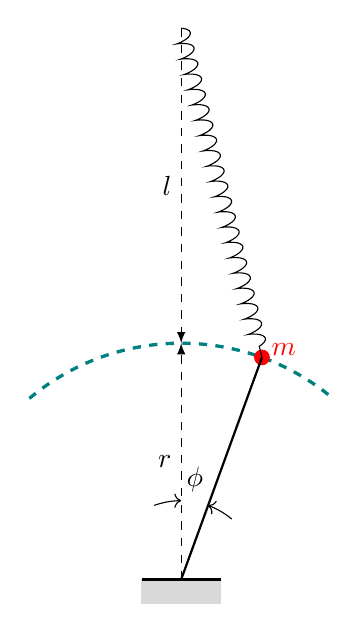
\begin{tikzpicture} %[=>stealth]
    \def\l{4};
    \def\r{3};
    \def\theta1{30};
    \def\theta2{40};

    \coordinate (O) at (0, 0);  
    \coordinate (A) at (0, {\l+\r});
    \coordinate (M) at (-1, 0);
    \coordinate (P1) at ({-\r * cos(110)}, {\r*sin(110)});
    \coordinate (P2) at ({\r * cos(110)}, {\r*sin(110)});
    \coordinate (P11) at ({\r * cos(130)}, {\r*sin(50)});
    \draw[dashed, -latex] (A) -- node [left] {$l$} (0, \r);
    \draw[dashed, -latex] (O) -- node [left] {$r$} (0, \r);
    \draw[very thick, teal, dashed] (P11) arc (130:50:{\r});
    \draw[->] ({1*cos(110)}, {1*sin(110)}) arc (110:90:1);
    \draw[->] ({1*cos(50)}, {1*sin(50)}) arc (50:70:1);
    \node[above ] at ({1*cos(80)}, {1*sin(80)}) {$\phi$};
  
    \fill[red] (P1) circle (0.1cm) node[above right, yshift=-0.3em] {$m$};
    \draw[decoration={aspect=0.3, segment length=2mm, amplitude=1mm,coil},decorate] (A) -- (P1); 
    \draw[thick] (O) -- (P1);
    \filldraw [fill=gray!30, draw=gray!30] (-0.5, 0) rectangle (0.5,-0.3);
    \draw[very thick] (-0.5, 0) -- (0.5, 0);  

\end{tikzpicture}
\end{document}
